\documentclass[manuscript]{acmart}

% ACM single-column manuscript-style student research manuscript.
% This is a generic ACM SIGCONF layout, not a claim of acceptance by an ACM venue.
\settopmatter{printacmref=false, printccs=false, printfolios=true}
\renewcommand\footnotetextcopyrightpermission[1]{}
\setcopyright{none}

\begin{document}

\title{Knowledge Cutoffs, Temporal Knowledge Boundaries, and Citation Reliability in Large Language Models: A Controlled Comparative Study of Explicit Publication-Date Instructions}

\author{Ankit Kumar}
\affiliation{%
  \institution{Indian Institute of Information Technology Allahabad}
  \country{India}
}

\begin{abstract}
Large language models (LLMs) can assist with literature synthesis, but generated references may violate a researcher's intended publication-date boundary. This study investigates whether adding an explicit publication-date instruction changes the temporal compliance of LLM-generated literature reviews. We conducted a controlled comparison of five matched prompt pairs (ten reviews). Condition A used a standard literature-review prompt; Condition B added an instruction to include only scholarly works published on or before 31 December 2024, inclusive, and to omit or flag uncertain dates rather than guess. Across 99 analyzed citation instances, Condition A contained 15 post-cutoff citations among 51 (29.41\%), while Condition B contained none among 48 (0\%). The mean paired reduction was 29.64 percentage points. A sensitivity analysis restricted to bibliographically matched references retained a mean paired reduction of 27.14 percentage points. All five pairs favored Condition B, but a two-sided exact sign test was not statistically significant at the conventional 0.05 level ($p=0.0625$). The results describe observable compliance with an explicit date constraint; they do not measure the model's internal training-data cutoff. The small sample and manual audit process require cautious interpretation.
\end{abstract}

\keywords{large language models, temporal knowledge boundaries, citation reliability, literature review generation, bibliographic verification, prompt instruction}

\maketitle
\pagestyle{plain}

\section{Introduction}
Large language models are increasingly used to summarize research, identify relevant work, and draft literature reviews. Prior work has examined automated literature-review generation and the reliability of references produced by conversational systems \cite{kasanishi2023scireviewgen,chelli2024hallucination}. However, fluent synthesis does not guarantee that a generated review respects a researcher's temporal scope. A review intended to represent the state of research at a historical date may include publications released after that date.

Temporal compliance and bibliographic reliability are related but distinct. A citation may refer to a real publication but fall outside the requested date range. Conversely, a reference may be within the date range but contain incorrect title, author, venue, or DOI metadata. Work on time-aware language modeling and retrieval-augmented generation provides context for treating temporal scope and source grounding as explicit system concerns \cite{dhingra2022timeaware,lewis2020rag}.

\subsection{Related work}
Research on temporal knowledge in language models has examined time-aware representations, temporal reasoning benchmarks, and the difficulty of maintaining knowledge as facts evolve. These studies motivate treating time as an explicit dimension of model behavior rather than assuming that a model's answers are temporally stable \cite{dhingra2022timeaware,cheng2024dated,wu2024continual,tan2023temporal,zhang2025time,pezik2025llmlagbench,prior2026oldfriend,zhang2026tempo}.

A second body of work studies factuality, hallucination, and the reliability of generated references. It includes methods for detecting uncertainty, surveys of hallucination, and empirical evaluations of citation quality in scholarly writing \cite{farquhar2024entropy,gao2023rag,huang2025hallucination,kalai2025hallucinate,wang2024editing,chelli2024hallucination}.

A third line of work focuses on retrieval and literature-review generation. Retrieval-augmented generation and active retrieval provide mechanisms for grounding generated text in external sources, while datasets and evaluations address automated review composition and scientific reference generation \cite{asai2024selfrag,jiang2023active,kasanishi2023scireviewgen,chen2025systematic,ramirez2025multi,scherbakov2025review,tang2025review,wu2025review}.

These strands establish relevant context, but they do not directly answer the narrow question tested here: whether adding an explicit publication-date boundary to a literature-review prompt changes the dates of the references actually emitted. The present study evaluates that prompt-level behavior without claiming to measure the model's internal training-data boundary.

This study tests a narrow intervention: adding an explicit publication-date boundary instruction to an otherwise standard literature-review prompt. The study does not attempt to infer the model's internal training cutoff. It evaluates the observable dates of references in generated outputs.

\subsection{Research question}
Does adding an explicit publication-date boundary instruction reduce post-cutoff citations in literature reviews generated by a large language model, and how does this affect bibliographic reliability?

\subsection{Contributions}
The study contributes (1) a small controlled comparison of standard and date-constrained prompting, (2) an instance-level temporal citation audit across five matched prompt pairs, and (3) a bibliographic-match sensitivity analysis that tests whether the descriptive pattern remains when unresolved references are excluded. The contribution is an empirical course-level comparison, not a new model architecture or a claim of broad generalization.

\section{Methodology}
\subsection{Study design and conditions}
We used a controlled comparative design with five matched prompt pairs, identified as P01--P05, yielding ten generated literature reviews. Condition A used a standard literature-review prompt. Condition B used the same underlying task preceded by an explicit instruction to cite only scholarly works published on or before 2024-12-31 (inclusive), and to omit or flag uncertain publication dates rather than guess. Generation order was randomized using seed 2026. Reviews were generated manually through the ChatGPT user interface rather than through an API.

\subsection{Data collection and protocol deviation}
The ten generated review texts were retained as individual output files. The model selector label and visible settings were recorded in the generation log where available. The intended output length was 800--1,000 words; the generated reviews exceeded this target. The deviation was documented and the original outputs were not shortened after generation. Manual interface generation also means that the original model generations are not exactly reproducible from a deterministic command.

\subsection{Citation extraction and audit}
The initial extraction contained 100 candidate entries. One entry was commentary rather than a complete bibliographic reference, leaving 99 analyzed citation instances. Candidate references were assessed using bibliographic metadata checks and manual review. Audit labels were MATCH, PARTIAL\_MATCH, DOI\_MISMATCH, and NOT\_APPLICABLE. A failed DOI lookup was not treated as proof that a reference was fabricated. The audit also recognized that preprint and later proceedings versions can have different publication dates.

\subsection{Temporal classification}
The cutoff was 31 December 2024, inclusive. Each analyzed reference was classified by its candidate publication year as WITHIN\_CUTOFF, POST\_CUTOFF, or UNKNOWN\_DATE. The analysis records candidate publication years and does not imply that every date was independently confirmed from a primary publisher record. When a preprint and a later published version differed, the cited version was relevant to the temporal classification.

\subsection{Measures}
The primary metric was the post-cutoff citation rate:
\[
R_{post}=\frac{N_{post-cutoff}}{N_{dated}}\times 100.
\]
The secondary metric was the bibliographic match rate:
\[
R_{match}=\frac{N_{MATCH}}{N_{analyzed}}\times 100.
\]
We also calculated pair-level differences in post-cutoff rates and a sensitivity analysis restricted to references classified as MATCH. Because there were only five matched pairs, the analysis emphasizes descriptive effect sizes and the direction of paired differences. A two-sided exact sign test was used to summarize the direction across pairs.

\subsection{Reproducibility and analysis boundary}
The repository retains the ten generated review texts, extraction and audit CSVs, protocol documents, and a Python script that re-computes descriptive summaries and figures from the archived data. This script reproduces the analysis of the archived tables; it does not regenerate the original LLM outputs or independently adjudicate every manual audit decision.

\section{Results}
\subsection{Overall temporal compliance}
Table~\ref{tab:overall} reports the overall citation outcomes. Condition A contained 15 post-cutoff citations among 51 instances (29.41\%). Condition B contained no post-cutoff citations among 48 instances (0\%).

\begin{table}[t]
\caption{Overall temporal and bibliographic outcomes}
\label{tab:overall}
\centering
\begin{tabular}{lrr}
\toprule
Measure & A & B \\
\midrule
Citation instances & 51 & 48 \\
Within cutoff & 36 & 48 \\
Post cutoff & 15 & 0 \\
Unknown year & 0 & 0 \\
Post-cutoff rate & 29.41\% & 0.00\% \\
MATCH instances & 45 & 48 \\
Match rate & 88.24\% & 100.00\% \\
\bottomrule
\end{tabular}
\end{table}

\begin{figure}[t]
  \centering
  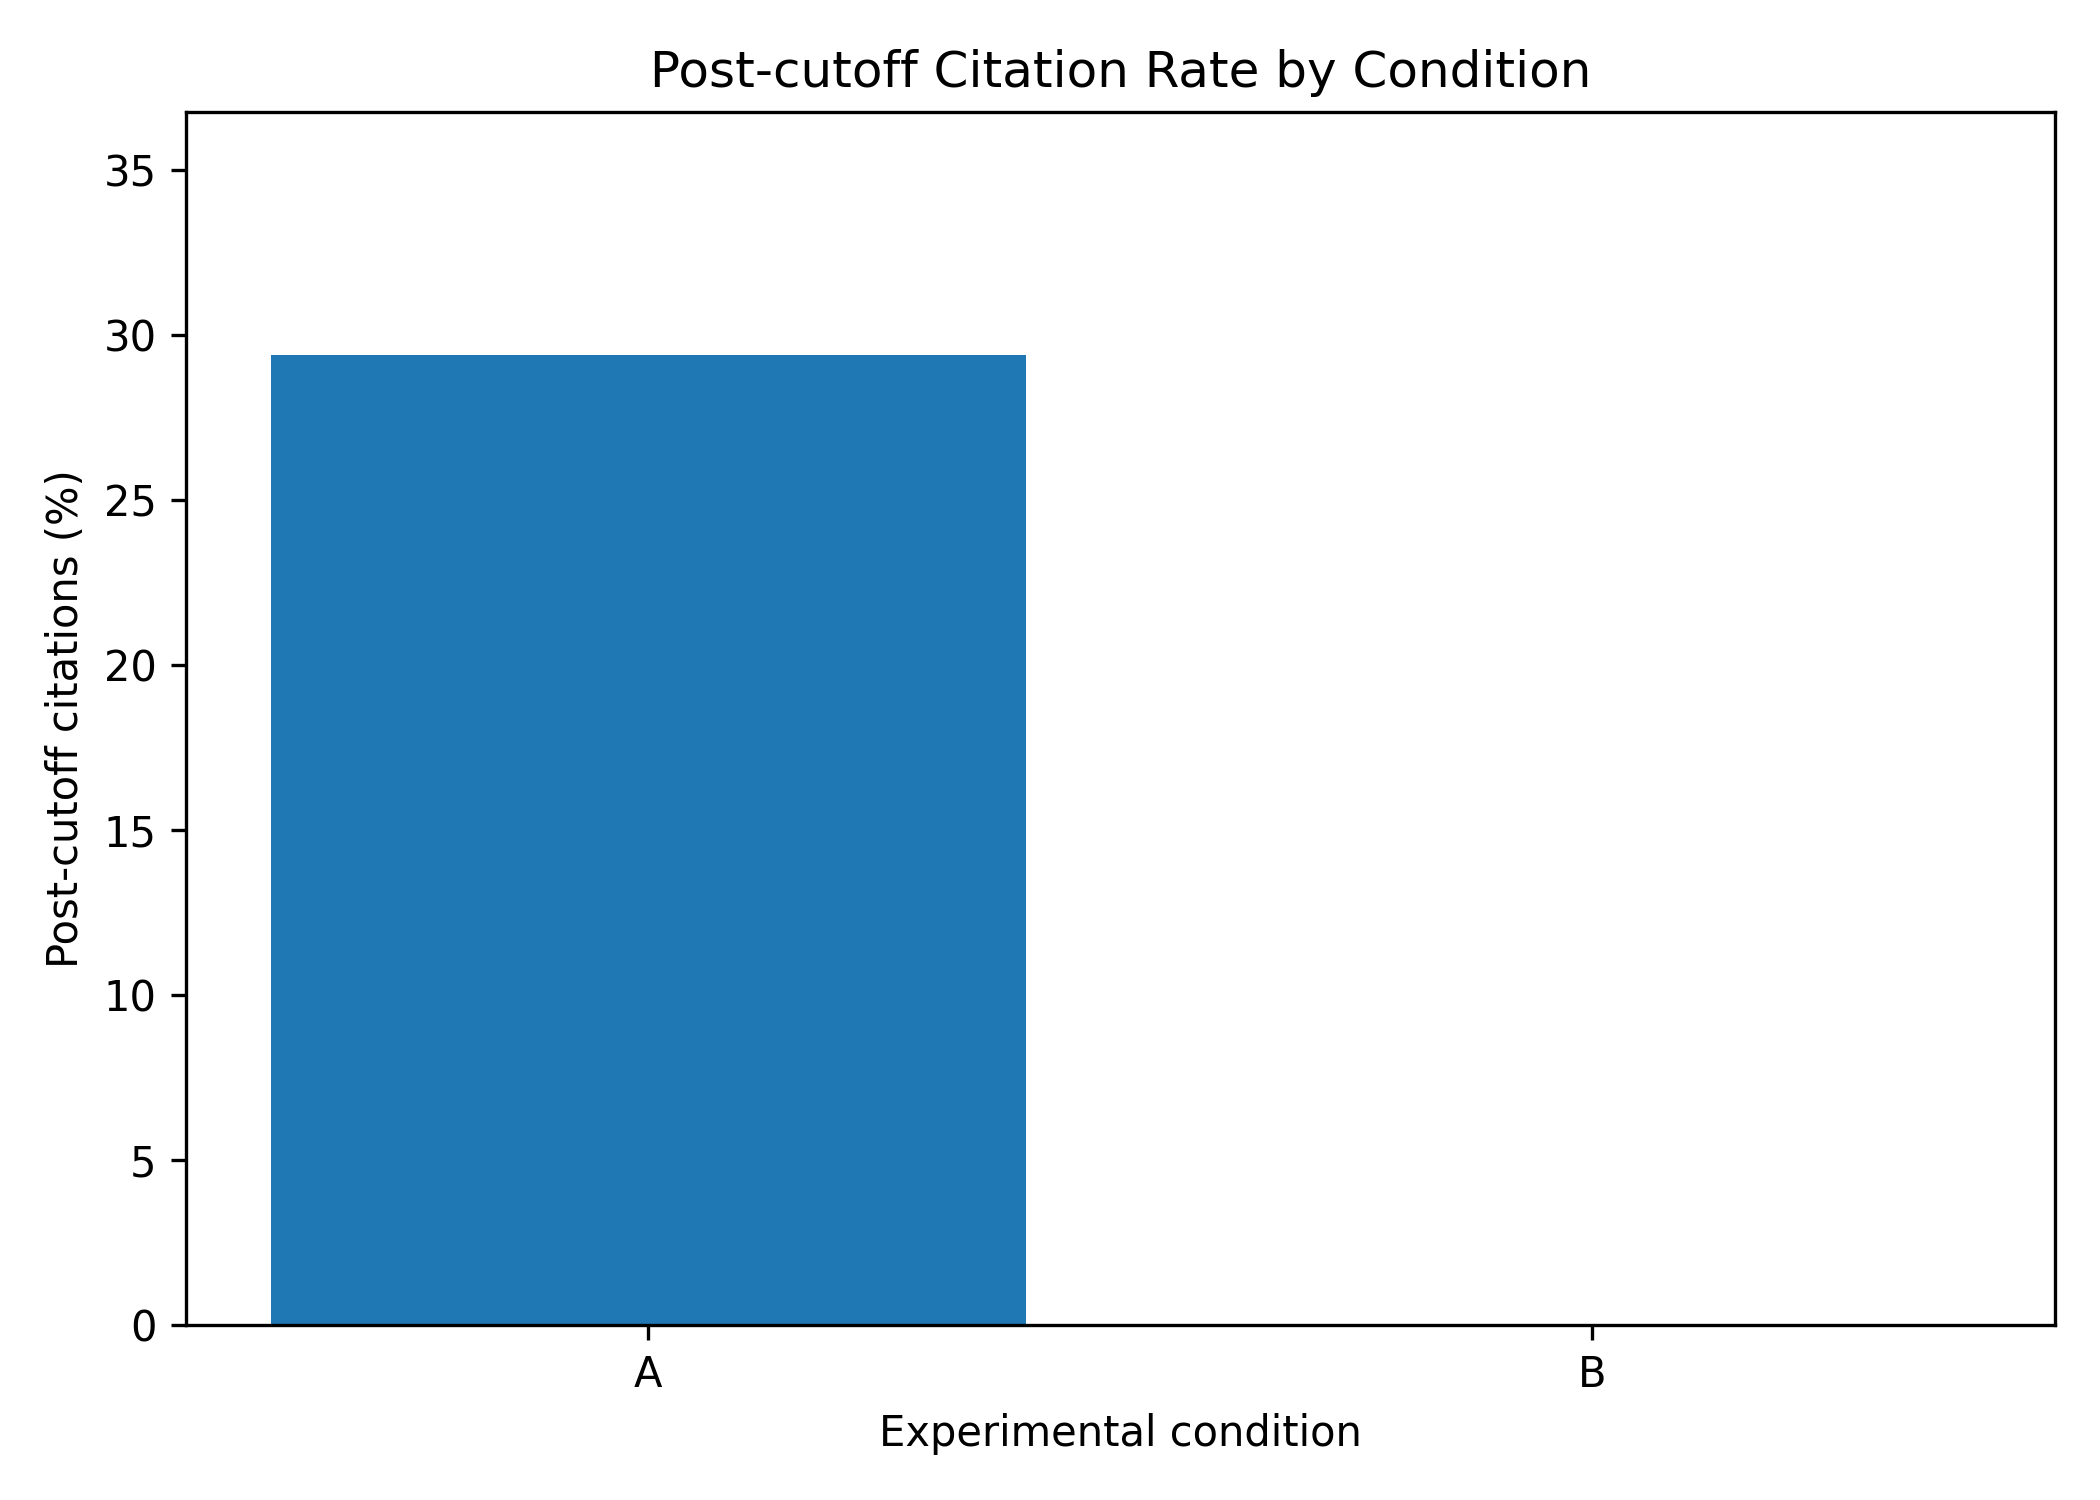
\includegraphics[width=\linewidth]{figures/figure1_overall_cutoff_rate.png}
  \caption{Overall post-cutoff citation rates under the two prompt conditions.}
  \Description{Bar chart comparing the post-cutoff citation rates: 29.41 percent for Condition A and zero percent for Condition B.}
  \label{fig:overall}
\end{figure}

\subsection{Matched-pair comparison}
The pair-specific post-cutoff rates for Condition A were 30.00\%, 30.00\%, 30.00\%, 18.18\%, and 40.00\%; all corresponding Condition B rates were 0\%. The mean paired reduction was 29.64 percentage points. The two-sided exact sign test yielded $p=0.0625$, which does not meet the conventional $\alpha=0.05$ threshold.

\begin{table}[t]
\caption{Post-cutoff rates by matched prompt pair}
\label{tab:paired}
\centering
\begin{tabular}{lrrr}
\toprule
Pair & A & B & Reduction (pp) \\
\midrule
P01 & 30.00\% & 0.00\% & 30.00 \\
P02 & 30.00\% & 0.00\% & 30.00 \\
P03 & 30.00\% & 0.00\% & 30.00 \\
P04 & 18.18\% & 0.00\% & 18.18 \\
P05 & 40.00\% & 0.00\% & 40.00 \\
\midrule
Mean & 29.64\% & 0.00\% & 29.64 \\
\bottomrule
\end{tabular}
\end{table}

\begin{figure}[t]
  \centering
  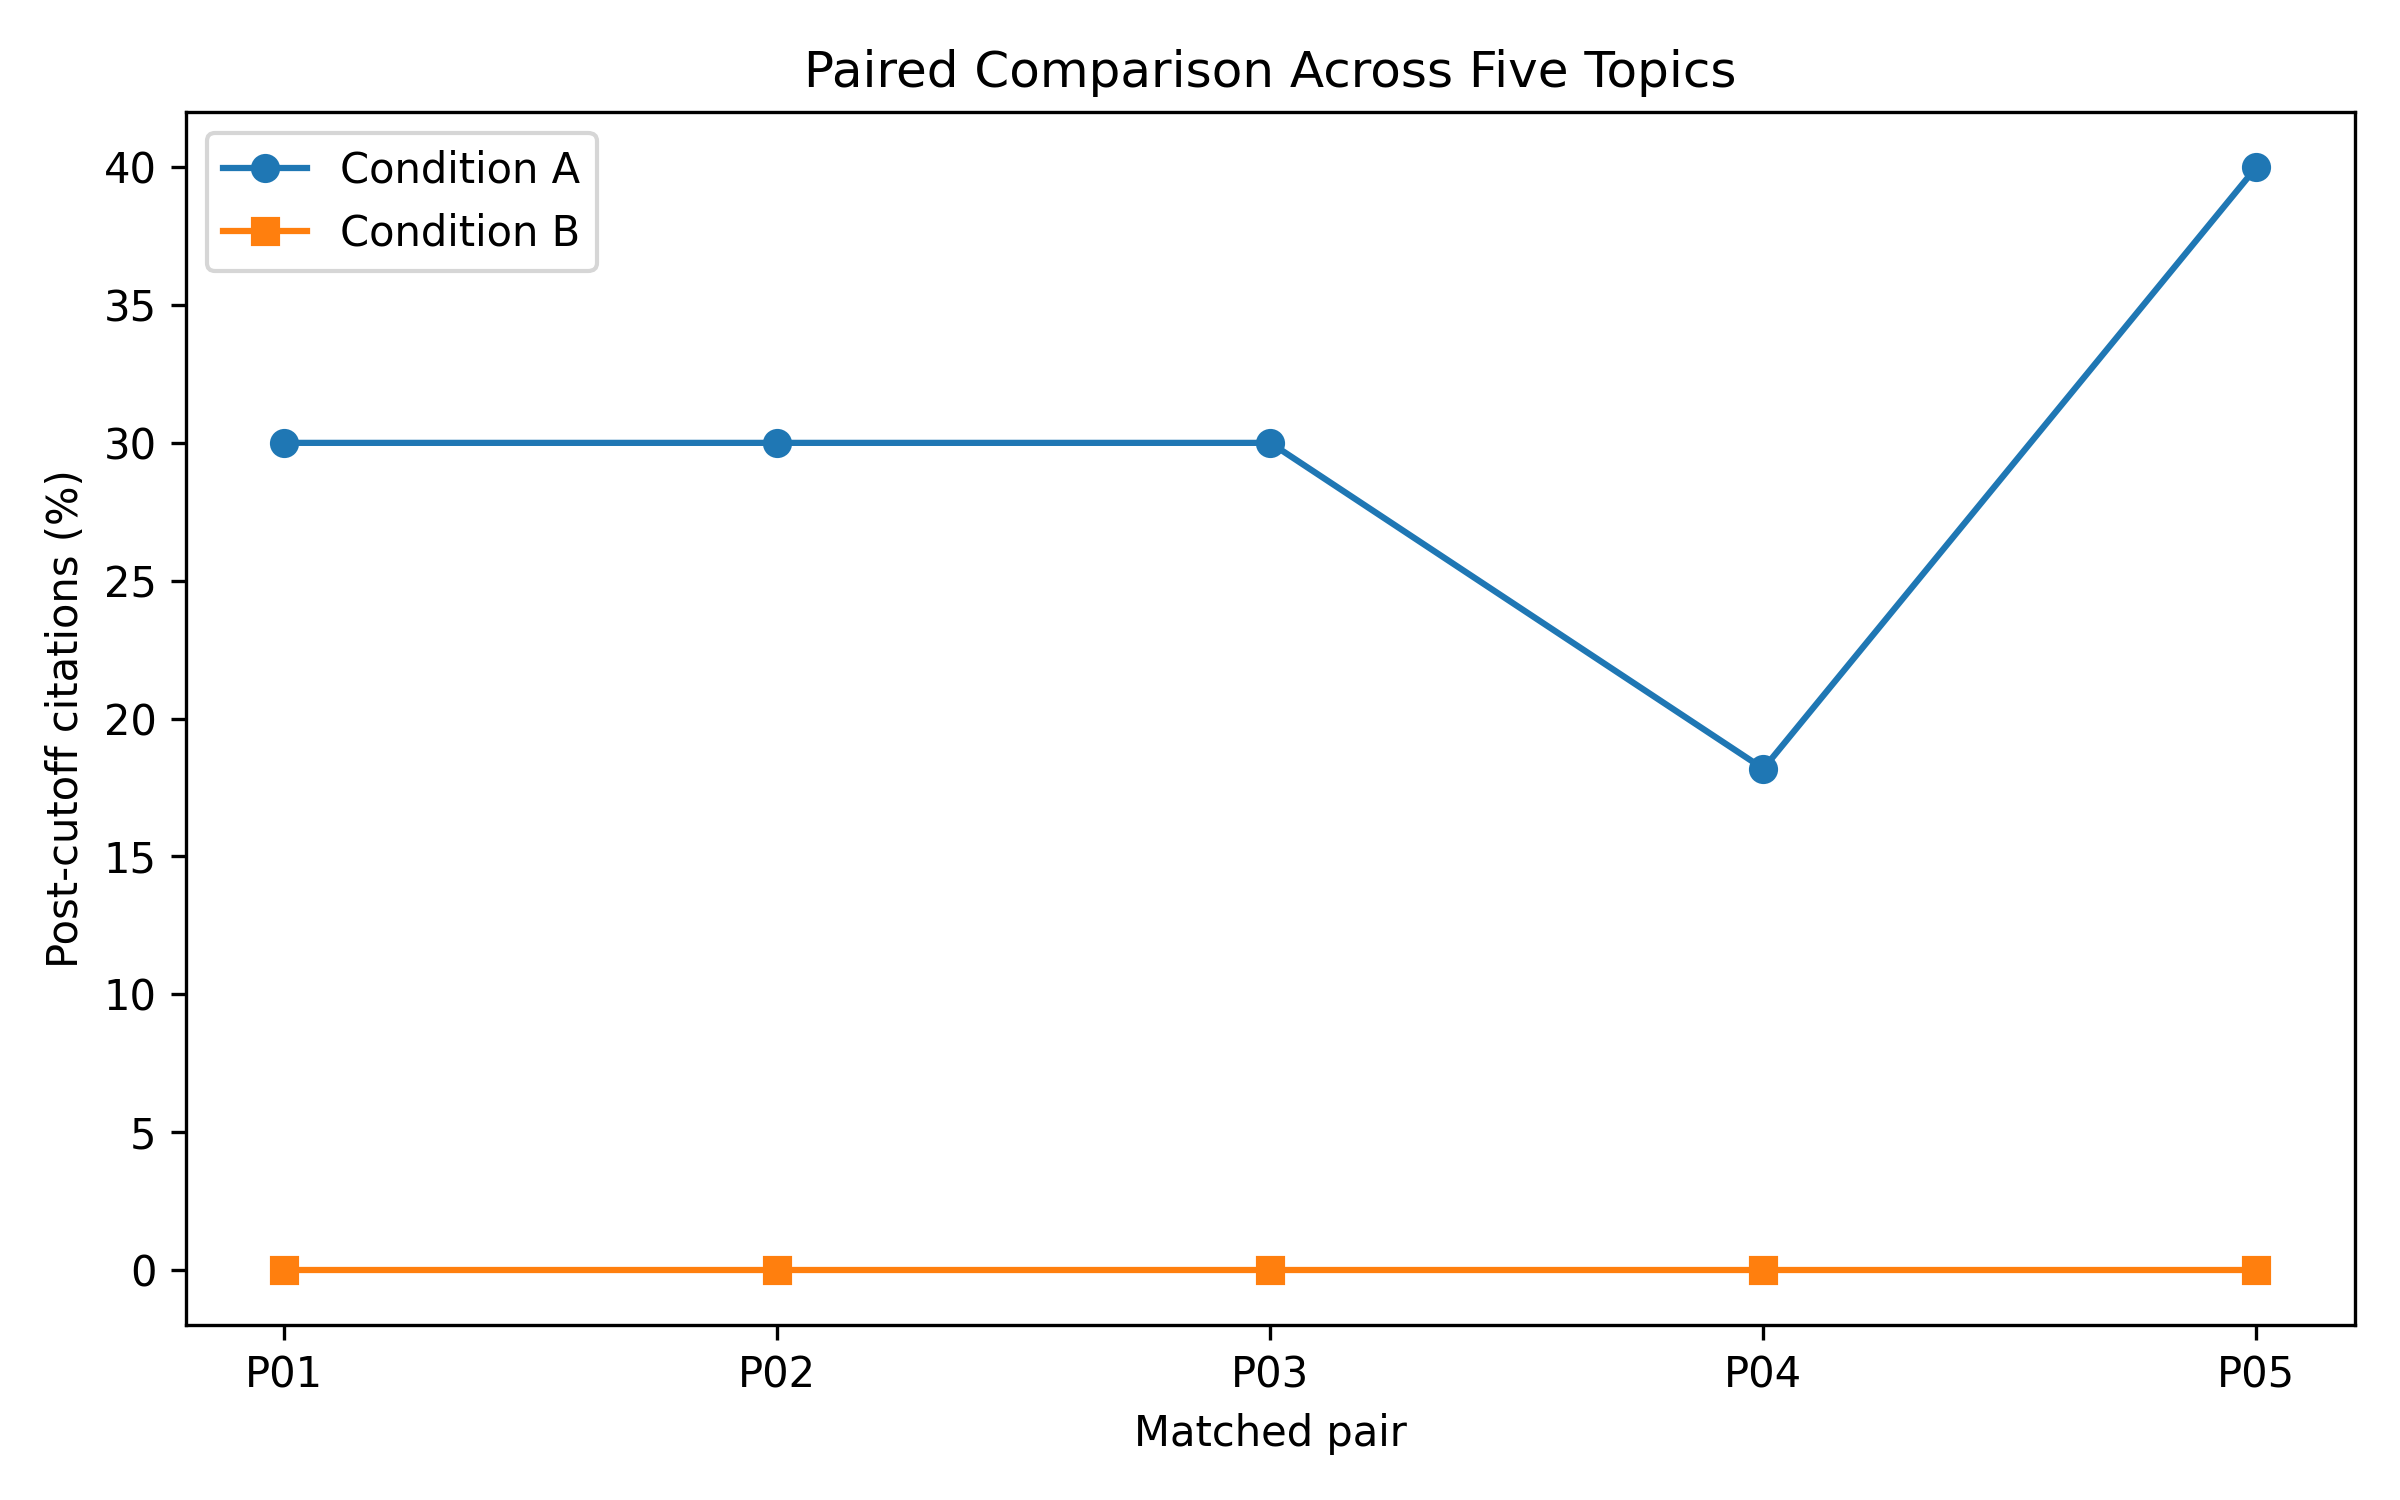
\includegraphics[width=\linewidth]{figures/figure2_paired_comparison.png}
  \caption{Post-cutoff citation rates for each matched prompt pair.}
  \Description{Paired comparison plot showing a positive post-cutoff rate in each Condition A review and zero in each Condition B review.}
  \label{fig:paired}
\end{figure}

\subsection{Bibliographic audit and sensitivity analysis}
The 100 extracted candidates comprised 93 MATCH, five PARTIAL\_MATCH, one DOI\_MISMATCH, and one NOT\_APPLICABLE entry. Excluding the non-reference commentary item left 99 analyzed citation instances. Condition A had 45 MATCH entries among 51 (88.24\%); Condition B had 48 among 48 (100\%). These are the recorded audit outcomes, not proof that every bibliographic field is error-free.

In the MATCH-only sensitivity analysis, Condition A retained 12 post-cutoff references among 45 confirmed matches (26.67\%), while Condition B retained none among 48. The mean paired reduction was 27.14 percentage points.

\begin{figure}[t]
  \centering
  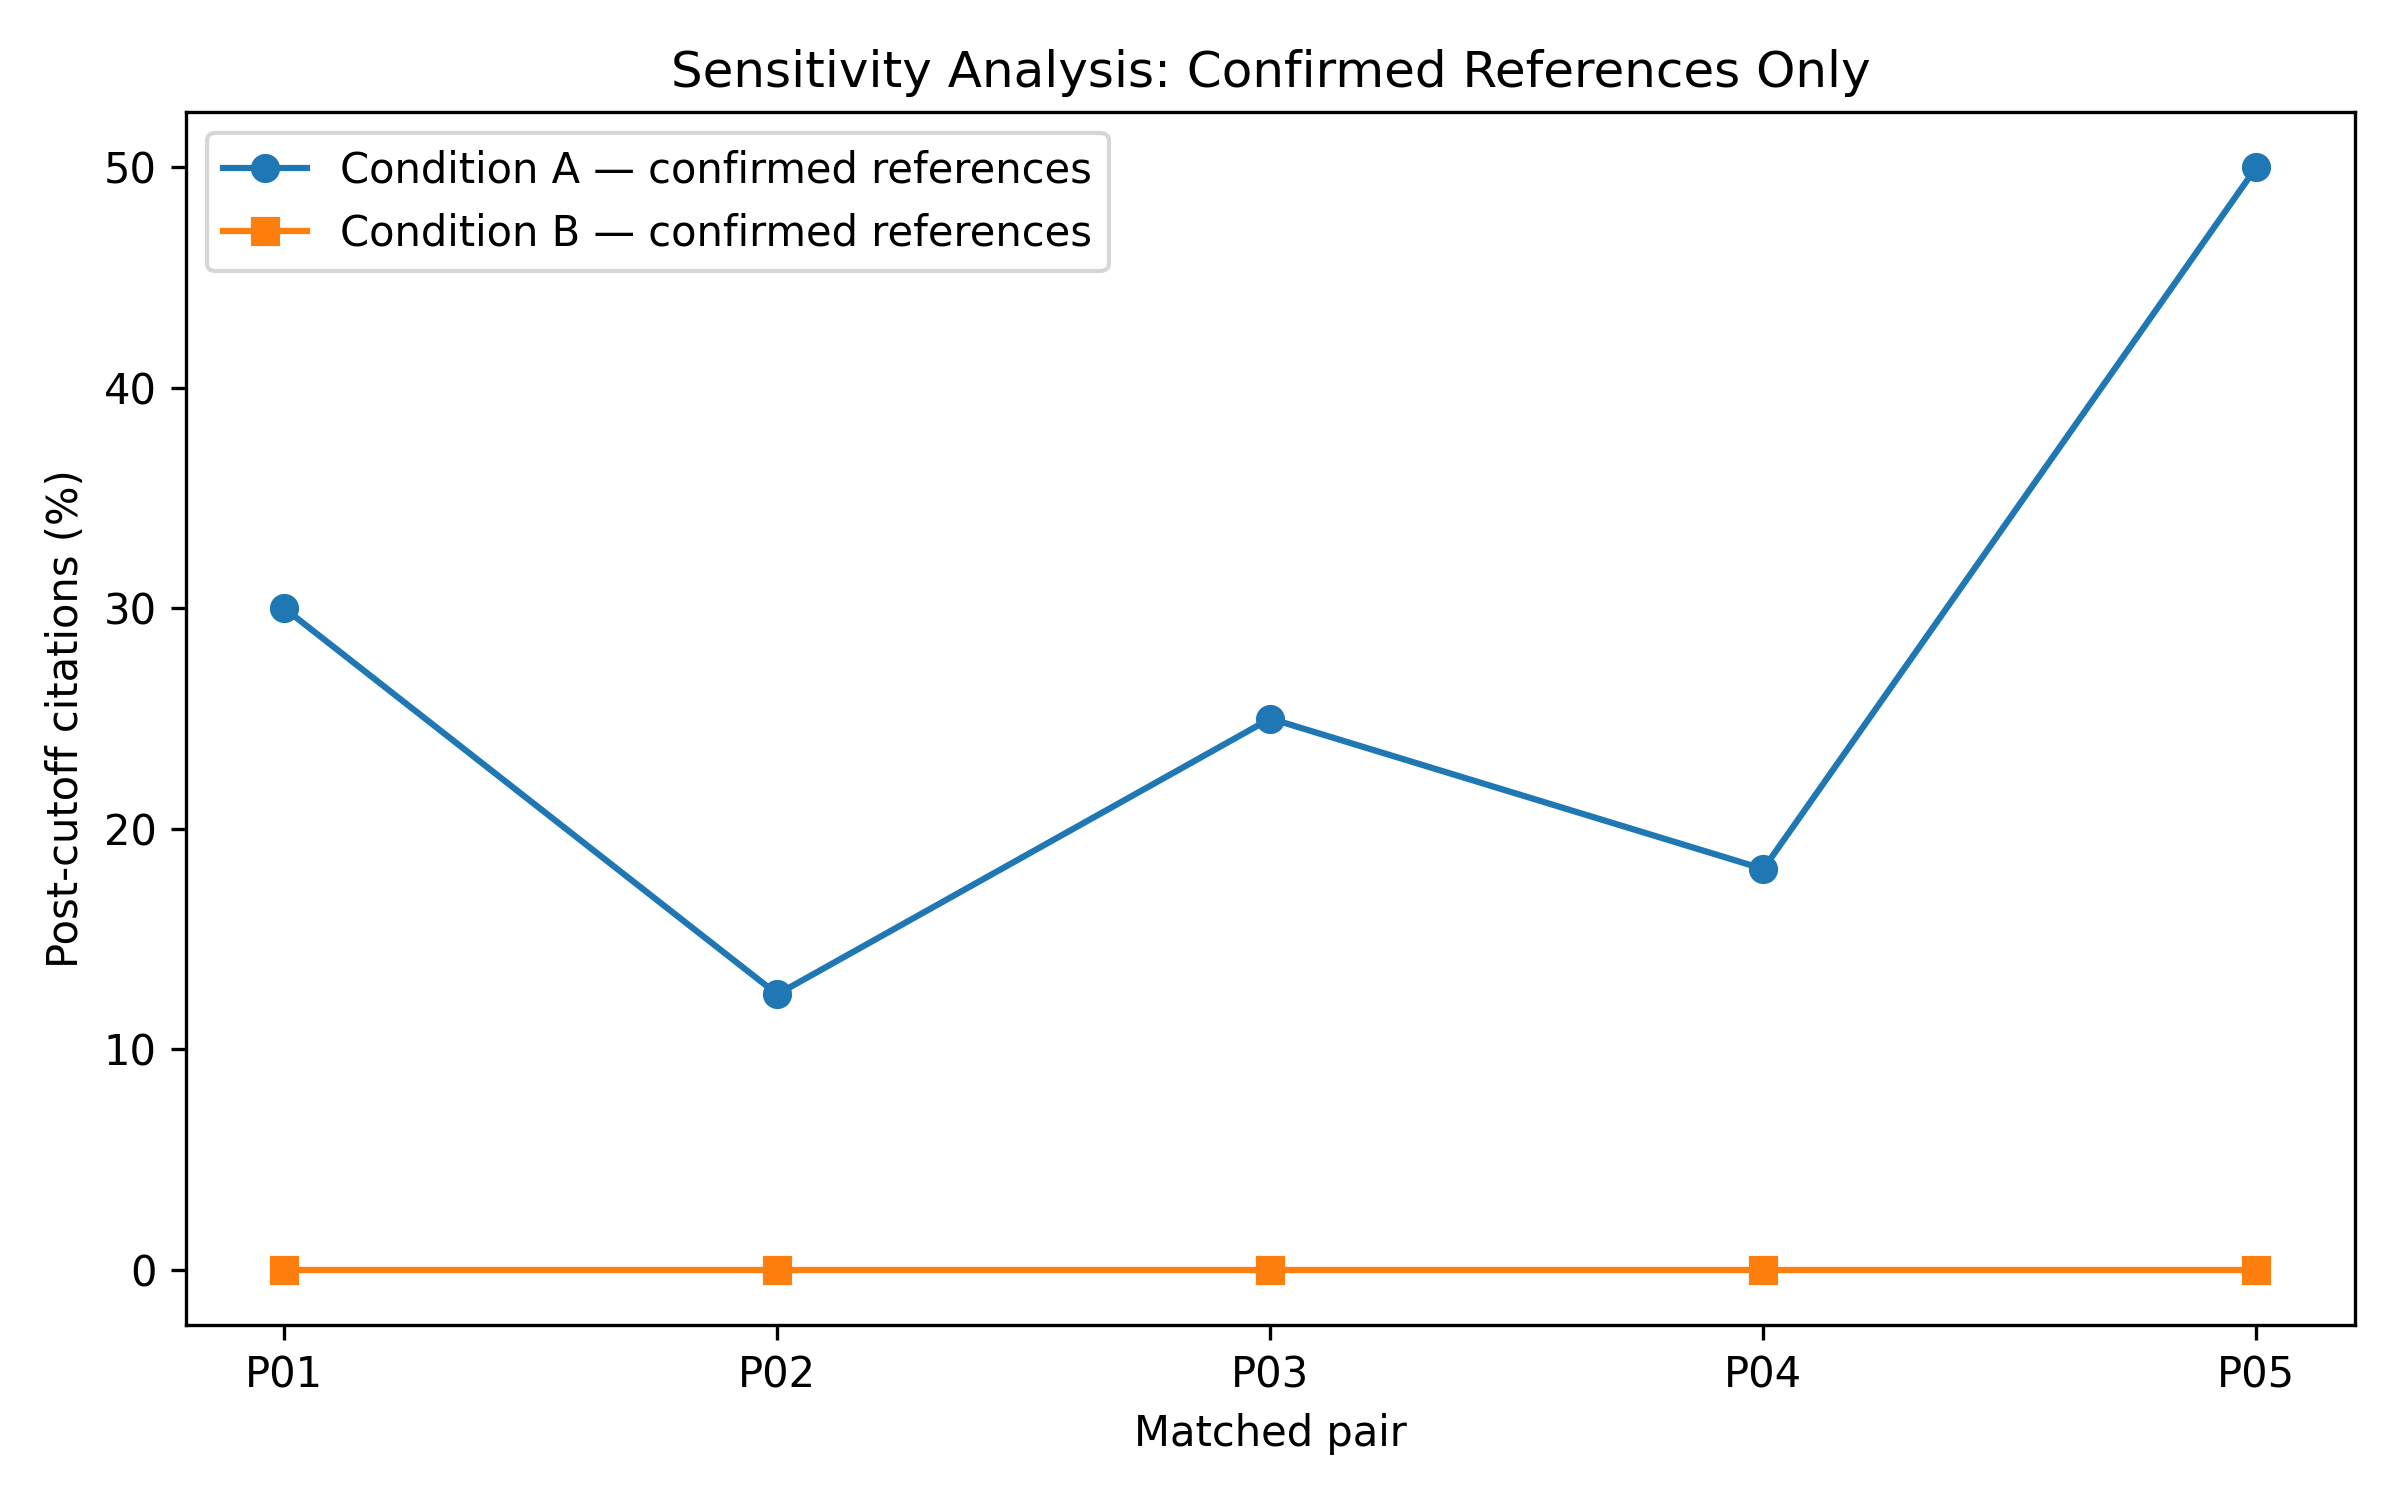
\includegraphics[width=\linewidth]{figures/figure3_sensitivity_analysis.png}
  \caption{Sensitivity analysis restricted to bibliographically matched references.}
  \Description{Sensitivity analysis chart comparing post-cutoff rates among MATCH references: 26.67 percent for Condition A and zero percent for Condition B.}
  \label{fig:sensitivity}
\end{figure}

\section{Discussion}
The observed pattern is consistent with the possibility that an explicit publication-date instruction improves temporal compliance in generated literature reviews. The direction of the difference was consistent across all five matched pairs and remained in the MATCH-only sensitivity analysis. This pattern is practically relevant because automated literature-review systems have been evaluated for reference generation and review composition, while reference accuracy remains a distinct concern from fluent text generation \cite{kasanishi2023scireviewgen,chelli2024hallucination}.

The evidence is not conclusive. The exact sign test was not statistically significant at the conventional 0.05 level, and five pairs provide limited statistical power. The difference in bibliographic match rates should also be interpreted cautiously: Condition B's higher match rate is an observed property of this small sample and does not establish that temporal instructions generally improve bibliographic accuracy.

A publication-date instruction is a prompt-level constraint, not a direct measurement of internal model knowledge. A post-cutoff reference may be introduced through retrieval, conversation context, model updates, or other mechanisms. Conversely, the absence of a post-cutoff reference does not demonstrate that the model lacks later information. Research on retrieval-augmented generation and temporal language modeling motivates this distinction between accessible information, time-conditioned outputs, and internal model parameters \cite{lewis2020rag,dhingra2022timeaware}.

\section{Limitations and Threats to Validity}
\textbf{Small sample.} The experiment contains five matched pairs and ten reviews. Results should not be generalized to all prompts, models, domains, or users.

\textbf{Single interface and model configuration.} Reviews were generated manually through one ChatGPT interface/model configuration. Interface settings and model availability may change over time.

\textbf{Output-length deviation.} All generated reviews exceeded the planned 800--1,000-word target. This protocol deviation was retained rather than corrected post hoc.

\textbf{Manual audit.} Bibliographic verification and publication-version classification involved manual decisions. Some entries were partial or inconsistent, and candidate publication years should not be conflated with independently verified publisher dates.

\textbf{Non-deterministic generation.} Manual UI generation is not a deterministic API-based reproduction. The archived script reproduces the analysis of stored data, not the original model generations.

\textbf{Construct validity.} The primary metric measures whether cited publication years fall after a stated cutoff. It does not measure the model's actual training-data cutoff, factual correctness of the review's narrative, completeness of literature coverage, or the causal mechanism behind the observed differences.

\section{Conclusion}
In this sample, the standard prompt condition produced a 29.41\% post-cutoff citation rate, while the explicit date-boundary condition produced 0\%. The mean paired reduction was 29.64 percentage points, and the MATCH-only sensitivity analysis retained a 27.14-point reduction. All five pairs favored the constrained prompt, but the two-sided exact sign test ($p=0.0625$) did not reach the conventional 0.05 threshold. The findings suggest that an explicit publication-date instruction may be a useful practical control for temporal scope, but it does not replace independent bibliographic verification and does not reveal the model's internal knowledge boundary. Larger studies across models, domains, prompt formulations, and repeated generations are needed.

\section*{Reproducibility Statement}
The companion repository contains the ten generated review texts, citation extraction and manual audit CSVs, prompt protocol, analysis script, and result figures. From the experiment directory, the archived-data analysis can be rerun using the documented Python command. Reproduction of the original manual ChatGPT generations is outside the scope of that script.

\bibliographystyle{ACM-Reference-Format}
\bibliography{references}

\end{document}
